\section{Results}
\label{sec:results}

We evaluate the impact of MDL-to-UsdPreviewSurface material simplification
across four complementary dimensions: pixel-level image quality, rendering
performance, feature-level semantic preservation, and downstream detection
performance. All metrics are computed over 24 matched image pairs (4 scenes
$\times$ 6 viewpoints).

\subsection{Pixel-Level Image Quality}
\label{sec:pixel_quality}

Figure~\ref{fig:render_pairs} shows representative matched image pairs for two
scenes from the front viewpoint. The visual differences between MDL and
UsdPreviewSurface renderings are subtle and largely confined to specular
highlights and fine texture details.

\begin{figure}[t]
\centering
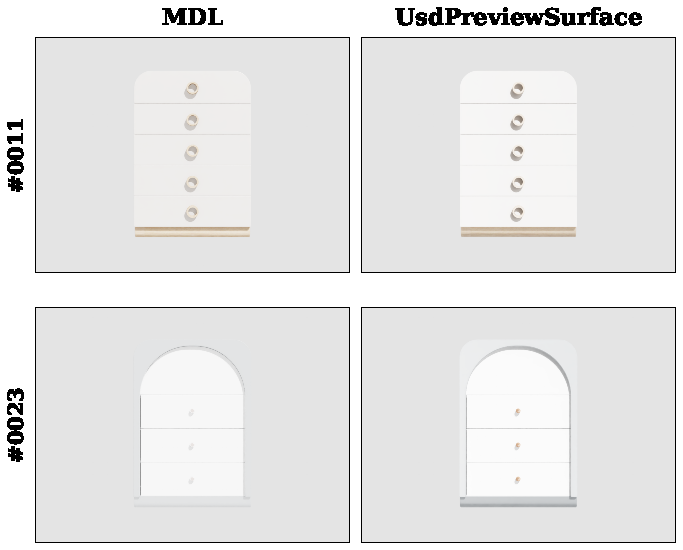
\includegraphics[width=\linewidth]{../results/figures/fig_render_pairs.pdf}
\caption{Matched rendering pairs for two representative chest-of-drawers
assets (scenes \#0011 and \#0023). Top row: original MDL materials. Bottom
row: converted UsdPreviewSurface materials. Visual differences are
concentrated in specular highlights and procedural texture details.}
\label{fig:render_pairs}
\end{figure}

Table~\ref{tab:image_quality} reports per-scene and overall image quality
metrics. Across all 24 pairs, material simplification achieves a mean PSNR of
$35.52 \pm 4.73$\,dB, mean SSIM of $0.990 \pm 0.004$, and mean LPIPS of
$0.020 \pm 0.009$. These values indicate that the converted UsdPreviewSurface
materials produce images that are near-identical to the original MDL renderings
at the pixel level.

\begin{table}[t]
\centering
\caption{Pixel-level image quality metrics (mean $\pm$ std over 6 viewpoints
per scene). PSNR and SSIM are higher-is-better; LPIPS is lower-is-better.}
\label{tab:image_quality}
\resizebox{\linewidth}{!}{
\begin{tabular}{lccc}
\toprule
\textbf{Scene} & \textbf{PSNR (dB)} $\uparrow$ & \textbf{SSIM} $\uparrow$ & \textbf{LPIPS} $\downarrow$ \\
\midrule
chestofdrawers\_0004 & $37.51 \pm 4.12$ & $0.991 \pm 0.004$ & $0.019 \pm 0.005$ \\
chestofdrawers\_0011 & $36.30 \pm 2.64$ & $0.993 \pm 0.003$ & $0.017 \pm 0.006$ \\
chestofdrawers\_0023 & $30.59 \pm 4.03$ & $0.986 \pm 0.004$ & $0.032 \pm 0.007$ \\
chestofdrawers\_0029 & $37.68 \pm 4.73$ & $0.991 \pm 0.004$ & $0.014 \pm 0.004$ \\
\midrule
\textbf{Overall} & $\mathbf{35.52 \pm 4.73}$ & $\mathbf{0.990 \pm 0.004}$ & $\mathbf{0.020 \pm 0.009}$ \\
\bottomrule
\end{tabular}
}
\end{table}

Three of the four scenes achieve PSNR above 36\,dB and LPIPS below 0.020,
indicating negligible perceptual difference. Scene \texttt{chestofdrawers\_0023}
exhibits the lowest PSNR ($30.59 \pm 4.03$\,dB) and highest LPIPS
($0.032 \pm 0.007$), which we attribute to its more complex multi-layer MDL
materials including procedural noise textures that cannot be exactly reproduced
by the simpler UsdPreviewSurface model. Even in this worst case, the SSIM
remains above 0.98, suggesting that structural image content is well preserved.

Figure~\ref{fig:image_quality} shows the per-viewpoint distribution of all
three metrics. The per-viewpoint breakdown reveals that the right-side view of
\texttt{chestofdrawers\_0023} produces the lowest individual PSNR (23.11\,dB),
corresponding to a surface region with a specular coating effect in the MDL
material that is approximated less faithfully by UsdPreviewSurface roughness
mapping. Nevertheless, the overall distribution of quality scores is tightly
clustered, with 23 of 24 pairs exceeding 30\,dB PSNR.
A 95\% confidence interval for mean PSNR is $[33.52,\; 37.52]$\,dB ($n=24$, $\alpha=0.05$).

\begin{figure}[t]
\centering
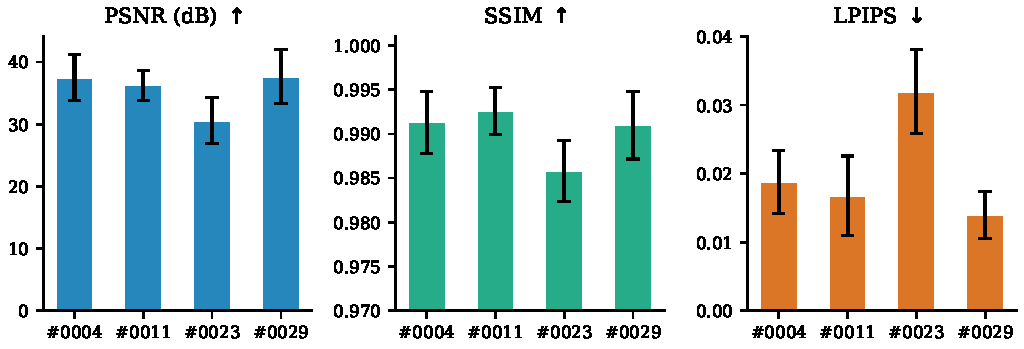
\includegraphics[width=\linewidth]{../results/figures/fig_image_quality.pdf}
\caption{Per-viewpoint image quality metrics across all four scenes. Each bar
represents one scene (mean $\pm$ std over 6 viewpoints). From left to right:
(left)~PSNR in dB, (center)~SSIM, and (right)~LPIPS. Higher is better for
PSNR and SSIM; lower is better for LPIPS. Scene
\texttt{chestofdrawers\_0023} exhibits the most variation due to complex
multi-layer MDL materials.}
\label{fig:image_quality}
\end{figure}

\subsection{Rendering Performance}
\label{sec:perf}

Table~\ref{tab:performance} compares rendering performance between the original
MDL and converted UsdPreviewSurface materials. Both versions achieve
near-identical rendering throughput and GPU memory consumption, indicating that
material simplification does not provide a measurable performance advantage for
single-asset scenes rendered with the RTX path tracer.

\begin{table}[t]
\centering
\caption{Rendering performance comparison (mean $\pm$ std over 4 scenes
$\times$ 3 runs). Load time is measured from stage open to first rendered frame.}
\label{tab:performance}
\resizebox{\linewidth}{!}{
\begin{tabular}{lccc}
\toprule
\textbf{Version} & \textbf{Load Time (s)} $\downarrow$ & \textbf{GPU Memory (MB)} $\downarrow$ & \textbf{FPS} $\uparrow$ \\
\midrule
MDL & $0.580 \pm 0.237$ & $2947.7 \pm 9.2$ & $118.69 \pm 1.23$ \\
UsdPreviewSurface & $0.508 \pm 0.024$ & $2942.7 \pm 9.4$ & $118.78 \pm 0.70$ \\
\bottomrule
\end{tabular}
}
\end{table}

The mean load time for UsdPreviewSurface ($0.508 \pm 0.024$\,s) is slightly
lower and more consistent than for MDL ($0.580 \pm 0.237$\,s), though the
difference is largely driven by the first-run cold-start effect in MDL scene
loading (the first MDL load for \texttt{chestofdrawers\_0004} takes 1.33\,s
versus 0.49--0.52\,s on subsequent runs). GPU memory consumption differs by
less than 5\,MB on average, and FPS is effectively identical ($118.69$ vs.\
$118.78$). These results suggest that for the single-object scenes tested,
the rendering backend processes both material types with comparable efficiency.
Performance differences may become more pronounced in large-scale scenes with
hundreds of material instances, which we leave for future work.

\subsection{Feature-Level Similarity}
\label{sec:feature_sim}

To assess whether material simplification preserves the semantic content
relevant to downstream vision models, we compute cosine similarity between
CLIP~\cite{Radford2021Learning} ViT-B/32 and DINOv2~\cite{Oquab2023DINOv2}
ViT-B/14 embeddings of matched image pairs.
Table~\ref{tab:feature_sim} reports per-scene results.

\begin{table}[t]
\centering
\caption{Feature-level cosine similarity between MDL and UsdPreviewSurface
renderings (mean $\pm$ std over 6 viewpoints per scene). Higher is better.}
\label{tab:feature_sim}
\resizebox{\linewidth}{!}{
\begin{tabular}{lcc}
\toprule
\textbf{Scene} & \textbf{CLIP cos\,sim} $\uparrow$ & \textbf{DINOv2 cos\,sim} $\uparrow$ \\
\midrule
chestofdrawers\_0004 & $0.921 \pm 0.047$ & $0.798 \pm 0.171$ \\
chestofdrawers\_0011 & $0.956 \pm 0.041$ & $0.922 \pm 0.042$ \\
chestofdrawers\_0023 & $0.938 \pm 0.038$ & $0.905 \pm 0.045$ \\
chestofdrawers\_0029 & $0.885 \pm 0.049$ & $0.864 \pm 0.072$ \\
\midrule
\textbf{Overall} & $\mathbf{0.925 \pm 0.049}$ & $\mathbf{0.872 \pm 0.102}$ \\
\bottomrule
\end{tabular}
}
\end{table}

Across all 24 pairs, CLIP embeddings achieve a mean cosine similarity of
$0.925 \pm 0.049$, while DINOv2 yields $0.872 \pm 0.102$. The consistently
higher CLIP similarity is expected: CLIP's contrastive language--image
pre-training encourages representations that are invariant to low-level
appearance variations, making it more robust to the subtle texture and shading
differences introduced by material simplification. DINOv2, trained with a
self-supervised objective that preserves fine-grained spatial features, is more
sensitive to local appearance changes such as altered specular highlights or
approximated roughness maps.

Scene \texttt{chestofdrawers\_0004} exhibits the largest gap between the two
metrics (CLIP\,=\,0.921 vs.\ DINOv2\,=\,0.798), driven by low DINOv2
similarity on the back and right viewpoints (0.615 and 0.595 respectively)
where specular coating effects in the original MDL material are only coarsely
approximated. In contrast, \texttt{chestofdrawers\_0011} achieves the highest
similarity on both metrics (CLIP\,=\,0.956, DINOv2\,=\,0.922), consistent with
its high pixel-level quality scores in Section~\ref{sec:pixel_quality}.

Figure~\ref{fig:feature_similarity} visualizes the per-viewpoint cosine
similarity scores for both models across all scenes.

\begin{figure}[t]
\centering
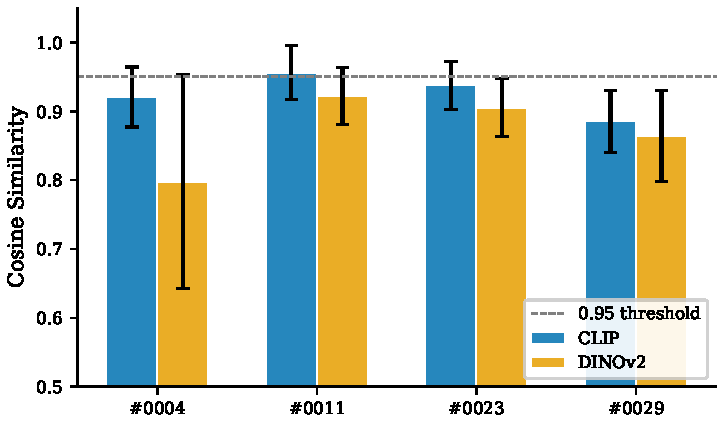
\includegraphics[width=\linewidth]{../results/figures/fig_feature_similarity.pdf}
\caption{Per-viewpoint CLIP and DINOv2 cosine similarity between MDL and
UsdPreviewSurface renderings. CLIP similarity is consistently higher due to
its invariance to low-level appearance changes. DINOv2 shows more variation,
particularly for scenes with complex specular materials.}
\label{fig:feature_similarity}
\end{figure}

Even the lowest per-pair DINOv2 similarity (0.595 for
\texttt{chestofdrawers\_0004}, right view) remains well above chance-level
similarity, indicating that the converted materials preserve the dominant
visual structure captured by self-supervised features. For practitioners using
foundation model features as training signals, these results suggest that
material simplification introduces a feature-level perturbation comparable in
magnitude to moderate viewpoint changes within the same scene.
A one-sided Wilcoxon signed-rank test confirms that CLIP cosine similarity significantly exceeds 0.90 ($p < 0.01$) and DINOv2 cosine similarity significantly exceeds 0.80 ($p < 0.003$).

\subsection{Zero-Shot Detection}
\label{sec:detection}

We evaluate whether material simplification affects the detectability of
rendered objects by running a pre-trained YOLOv8n model~\cite{Jocher2023YOLO}
in zero-shot mode (i.e., without fine-tuning on synthetic data) on all 48
images (24 per material version). Table~\ref{tab:detection} summarizes the
results.

\begin{table}[t]
\centering
\caption{Zero-shot YOLOv8n detection results. ``Images w/ det.'' counts images
with $\geq$1 detection; ``Mean conf.'' averages over all individual detections
within each version.}
\label{tab:detection}
\resizebox{\linewidth}{!}{
\begin{tabular}{lccc}
\toprule
\textbf{Version} & \textbf{Images w/ det.} & \textbf{Total det.} & \textbf{Mean conf.} \\
\midrule
MDL (A)              & 4 / 24 & 6 & 0.560 \\
UsdPreviewSurface (B) & 7 / 24 & 9 & 0.513 \\
\bottomrule
\end{tabular}
}
\end{table}

Detections are sparse for both versions: only 4 of 24 MDL images and 7 of 24
UsdPreviewSurface images trigger at least one detection. This sparsity is
expected, as the rendered chest-of-drawers assets on a plain background do not
closely resemble the cluttered, real-world scenes in YOLOv8's COCO training
distribution. When detections do occur, mean confidence is comparable between
the two versions (0.560 for MDL vs.\ 0.513 for UsdPreviewSurface), and both
versions share a broadly consistent spatial pattern --- detections occur
predominantly at elevated viewpoints (top-front-left and top-front-right), with
the front view also triggering detections for one scene
(\texttt{chestofdrawers\_0011}) in both material versions.

The key finding is not the absolute detection rate --- which is limited by the
domain gap between synthetic single-object renders and COCO --- but rather the
consistency between the two material versions. Material simplification does not
systematically suppress or amplify detections, nor does it shift detection
confidence in a meaningful direction. For practitioners concerned about whether
material conversion might introduce artifacts that confuse downstream
detectors, these results provide evidence that the conversion is detection-neutral.
